% ------------------------------------------------------------------------
% ------------------------------------------------------------------------
% Modelo UFSC para Trabalhos Academicos (tese de doutorado, dissertação de
% mestrado) utilizando a classe abntex2
%
% Autor: Alisson Lopes Furlani
% 	Modificações:
%	- 27/08/2019: Alisson L. Furlani, add 'glossaries' package
%   - 30/10/2019: Alisson L. Furlani, adjusted some spacing errors and changed math fonts
%   - 17/01/2020: Alisson L. Furlani, updated certification page
%   - 07/02/2020: Alisson L. Furlani, fixed table counter bug
%   - 11/03/2020: Alisson L. Furlani, changed greek letters in math and fixed citation style
% ------------------------------------------------------------------------
% ------------------------------------------------------------------------


\documentclass[
	% -- opções da classe memoir --
	12pt,				% tamanho da fonte
	openright,			% capítulos começam em pág ímpar (insere página vazia caso preciso)
	twoside,			% para impressão no anverso. Oposto a twoside
	a4paper,			% tamanho do papel. 
	% -- opções da classe abntex2 --
	chapter=TITLE,		% títulos de capítulos convertidos em letras maiúsculas
	section=TITLE,		% títulos de seções convertidos em letras maiúsculas
	%subsection=TITLE,	% títulos de subseções convertidos em letras maiúsculas
	%subsubsection=TITLE,% títulos de subsubseções convertidos em letras maiúsculas
	% -- opções do pacote babel --
	brazil,
	english			% idioma adicional para hifenização
	%french,				% idioma adicional para hifenização
	%spanish,			% idioma adicional para hifenização
	% brazil				% o último idioma é o principal do documento
	]{abntex2}


\usepackage{setup/ufscthesisA4-alf}
\usepackage{lipsum}

% Serif fonts
%\usepackage{mathptmx}
\usepackage{palatino}
%\usepackage[lining]{ebgaramond}
\usepackage{float}
\usepackage{multirow}
% \usepackage{fourier}
% \usepackage[T1]{fontenc}

%\usepackage{librebaskerville}
%\usepackage[T1]{fontenc}

% \usepackage{librecaslon}
% \usepackage[T1]{fontenc}

% Sans Serif fonts
\usepackage[defaultsans]{lato}
\usepackage{arydshln}
\usepackage{inconsolata}

\setlength\dashlinedash{1pt}
\setlength\dashlinegap{2pt}
%\usepackage[defaultsans]{cmbright}


\newcommand{\blue}[1]{{\color{blue}#1}}
% Text font
\renewcommand{\familydefault}{\rmdefault}
\renewcommand{\ttdefault}{lmtt} 
\newcommand{\citechapter}[1]{Chapter \ref{#1}}
\newcommand{\todo}[1]{\noindent{\color{blue}\textbf{TODO:} #1}}

\addbibresource{aftertext/references.bib} % Seus arquivos de referências

% ---
% Filtering and Mapping Bibliographies
% ---
\DeclareSourcemap{
	\maps[datatype=bibtex]{
		% remove fields that are always useless
		\map{
			\step[fieldset=abstract, null]
			\step[fieldset=pagetotal, null]
		}
		% remove URLs for types that are primarily printed
%		\map{
%			\pernottype{software}
%			\pernottype{online}
%			\pernottype{report}
%			\pernottype{techreport}
%			\pernottype{standard}
%			\pernottype{manual}
%			\pernottype{misc}
%			\step[fieldset=url, null]
%			\step[fieldset=urldate, null]
%		}
		\map{
			\pertype{inproceedings}
			% remove mostly redundant conference information
			\step[fieldset=venue, null]
			\step[fieldset=eventdate, null]
			\step[fieldset=eventtitle, null]
			% do not show ISBN for proceedings
			\step[fieldset=isbn, null]
			% Citavi bug
			\step[fieldset=volume, null]
		}
	}
}
% ---

% ---
% Informações de dados para CAPA e FOLHA DE ROSTO
% ---
% FIXME Substituir 'Nome completo do autor' pelo seu nome.
\autor{Thiago Raulino Dal Pont}
% FIXME Substituir 'Título do trabalho' pelo título da trabalho.
%\titulo{Classification of legal documents and prediction of compensation based on Text Mining and Machine Learning}
\titulo{Representation, classification and regression techniques applied to legal judgments about immaterial damage due to failures in air  transport services}
% Representation, classification and regression applied to legal judgments about immaterial damage from air transport service failures

% FIXME Substituir 'Subtítulo (se houver)' pelo subtítulo da trabalho.  
% Caso não tenha substítulo, comente a linha a seguir.
%\subtitulo{subtítulo (se houver)}
\orientador{Prof. Jomi Fred Hübner, PhD.}
% \orientador[Orientadora]{Nome da orientadora, Dra.}
\coorientador{Prof. Aires José Rover, PhD.}
\ano{2021}
% FIXME Substituir '[dia] de [mês] de [ano]' pela data em que ocorreu sua defesa.
\data{28 de agosto de 2021}
% FIXME Substituir 'Local' pela cidade em que ocorreu sua defesa.
\local{Florianópolis}
\instituicaosigla{UFSC}
\instituicao{Universidade Federal de Santa Catarina}
\tipotrabalho{Dissertação}
\formacao{mestre em Engenharia de Automação e Sistemas}
\nivel{mestrado}
\programa{Programa de Pós-Gra\-du\-a\-ção em Engenharia de Automação e Sistemas}
\centro{Centro Tecnológico e Científico}
\preambulo
{%
\imprimirtipotrabalho~submetida ao \imprimirprograma~da \imprimirinstituicao para a obtenção do título de \imprimirformacao.
}
% ---

% ---
% Configurações de aparência do PDF final
% ---
% alterando o aspecto da cor azul
\definecolor{blue}{RGB}{41,5,195}
%\usepackage[a-1b]{pdfx}
% informações do PDF
\makeatletter
\hypersetup{
     	%pagebackref=true,
		pdftitle={\@title}, 
		pdfauthor={Thiago Raulino Dal Pont},
    	pdfsubject={\imprimirpreambulo},
	    pdfcreator={LaTeX with abnTeX2},
		pdfkeywords={UFSC, DAS, Machine Learning, Text Classification, Text Representation, Text Regression, Special Civel Court, Legal Judgments}, 
		colorlinks=true,       		% false: boxed links; true: colored links
    	linkcolor=black,%blue,          	% color of internal links
    	citecolor=black,%blue,        		% color of links to bibliography
    	filecolor=black,%magenta,      		% color of file links
		urlcolor=black,%blue,
		bookmarksdepth=4
}
\makeatother
% ---

% ---
% compila a lista de abreviaturas e siglas e a lista de símbolos
% ---

% Declaração das siglas
\siglalista{AI}{Artificial Intelligence}
\siglalista{ML}{Machine Learning}
\siglalista{BOW}{Bag of Words}
\siglalista{VSM}{Vector Space Model}
\siglalista{JEC}{Special Civel Court}
\siglalista{TM}{Text Mining}
\siglalista{TF}{Term Frequency}
\siglalista{TF-IDF}{Term Frequency-Inverse Document Frequency}
\siglalista{IDF}{Inverse Document Frequency}
\siglalista{DL}{Deep Learning}
\siglalista{JECs}{Special Civel Courts}
\siglalista{SRL}{Systematic Review of the Literature}
\siglalista{LDA}{Latent Dirichlet Allocation}
\siglalista{CNJ}{National Council of Justice}
\siglalista{GPT-3}{Generative Pre-trained Transformer-3}
\siglalista{NLP}{Natural Language Processing}
\siglalista{MI}{Mutual Information}
\siglalista{RFE}{Recursive Feature Elimination}
\siglalista{PCA}{Principal Component Analysis}
\siglalista{PC}{Principal Component}
\siglalista{RBF}{Radial Basis Function}
\siglalista{NMF}{Non-negative Matrix Factorization}
\siglalista{CNN}{Convolutional Neural Network}
\siglalista{LSTM}{Long-Short Term Memory}
\siglalista{Bi-LSTM}{Bidirectional Long-Short Term Memory}
\siglalista{CBOW}{Continuous Bag of Words}
\siglalista{BERT}{Bidirectional Encoder Representations from Transformers}
\siglalista{ELMo}{Embeddings from Language Model}
\siglalista{AB}{AdaBoost}
\siglalista{XGB}{XGBoosting}
\siglalista{RF}{Random Forest}
\siglalista{LR}{Logistic Regression}
\siglalista{kNN}{k Nearest Neighbors}
\siglalista{SVM}{Support Vector Machine}
\siglalista{NN}{feed-forward Neural Networks}
\siglalista{GB}{Gradient Boosting}
\siglalista{BG}{Bagging}
\siglalista{RNN}{Recurrent Neural Network}
\siglalista{DT}{Decision Tree}
\siglalista{NB}{Na\"ive Bayes}
\siglalista{TP}{True Positive}
\siglalista{TN}{True Negative}
\siglalista{UFSC}{Federal University of Santa Catarina}
\siglalista{XAI}{Explainable Artificial Intelligence}
\siglalista{FN}{False Negative}
\siglalista{FP}{False Positive}
\siglalista{t-SNE}{t-distributed Stochastic Neighbor Embedding}
\siglalista{RMSE}{Root Mean Square Error}
\siglalista{MAE}{Mean Absolute Error}
\siglalista{$R^2$}{Coefficient of Determination}
\siglalista{STF}{Federal Supreme Court}
\siglalista{STJ}{Superior Court of Justice}
\siglalista{TJ-SC}{State Court of Santa Catarina}
\siglalista{EGOV}{E-government, Digital Inclusion and Knowledge Society}
\siglalista{RG}{Ridge}
\siglalista{LOO}{Leave-One-Out}
\siglalista{LSA}{Latent Semantic Analysis}
\siglalista{SOTA}{State of the Art}
\siglalista{POS}{Part-of-Speech}
\siglalista{eJRM}{Justice Relationship Management}
\siglalista{GR}{General Repercussion}
\siglalista{UnB}{University of Brasilia}
\siglalista{NLTK}{Natural Language Toolkit}
\siglalista{GPU}{Graphics Processing Unit}
\siglalista{TJ}{State Court}
\siglalista{RTF}{Rich Text Format}
\siglalista{OCR}{Optical Character Recognition}
\siglalista{PDF}{Portable Document Format}
\siglalista{SG}{Skipgram}
\siglalista{AELE}{Attributes Extracted by the Legal Expert}
\siglalista{EV}{Ensemble Voting}
\siglalista{EN}{Elastic Net}

% Declaração dos simbolos
\simbololista{C}{\ensuremath{C}}{Circunferência de um círculo}
\simbololista{pi}{\ensuremath{\pi}}{Número pi} 
\simbololista{r}{\ensuremath{r}}{Raio de um círculo}
\simbololista{A}{\ensuremath{A}}{Área de um círculo}

% compila a lista de abreviaturas e siglas e a lista de símbolos
\makenoidxglossaries 
%\makeglossaries
% ---

% ---
% compila o indice
% ---
\makeindex
% ---



% ----
% Início do documento
% ----
\begin{document}

% Seleciona o idioma do documento (conforme pacotes do babel)
\renewcommand{\arraystretch}{1.3}
\selectlanguage{english}
%\selectlanguage{brazil}

% Retira espaço extra obsoleto entre as frases.
\frenchspacing 

% Espaçamento 1.5 entre linhas
\OnehalfSpacing

% Corrige justificação
%\sloppy

% ----------------------------------------------------------
% ELEMENTOS PRÉ-TEXTUAIS
% ----------------------------------------------------------
% \pretextual %a macro \pretextual é acionado automaticamente no início de \begin{document}
% ---
% Capa, folha de rosto, ficha bibliografica, errata, folha de apróvação
% Dedicatória, agradecimentos, epígrafe, resumos, listas
% ---
% ---
% Capa
% ---
\imprimircapa
% ---

% ---
% Folha de rosto
% (o * indica que haverá a ficha bibliográfica)
% ---
\imprimirfolhaderosto*
% ---

% ---
% Inserir a ficha bibliografica
% ---
% http://ficha.bu.ufsc.br/
\begin{fichacatalografica}
	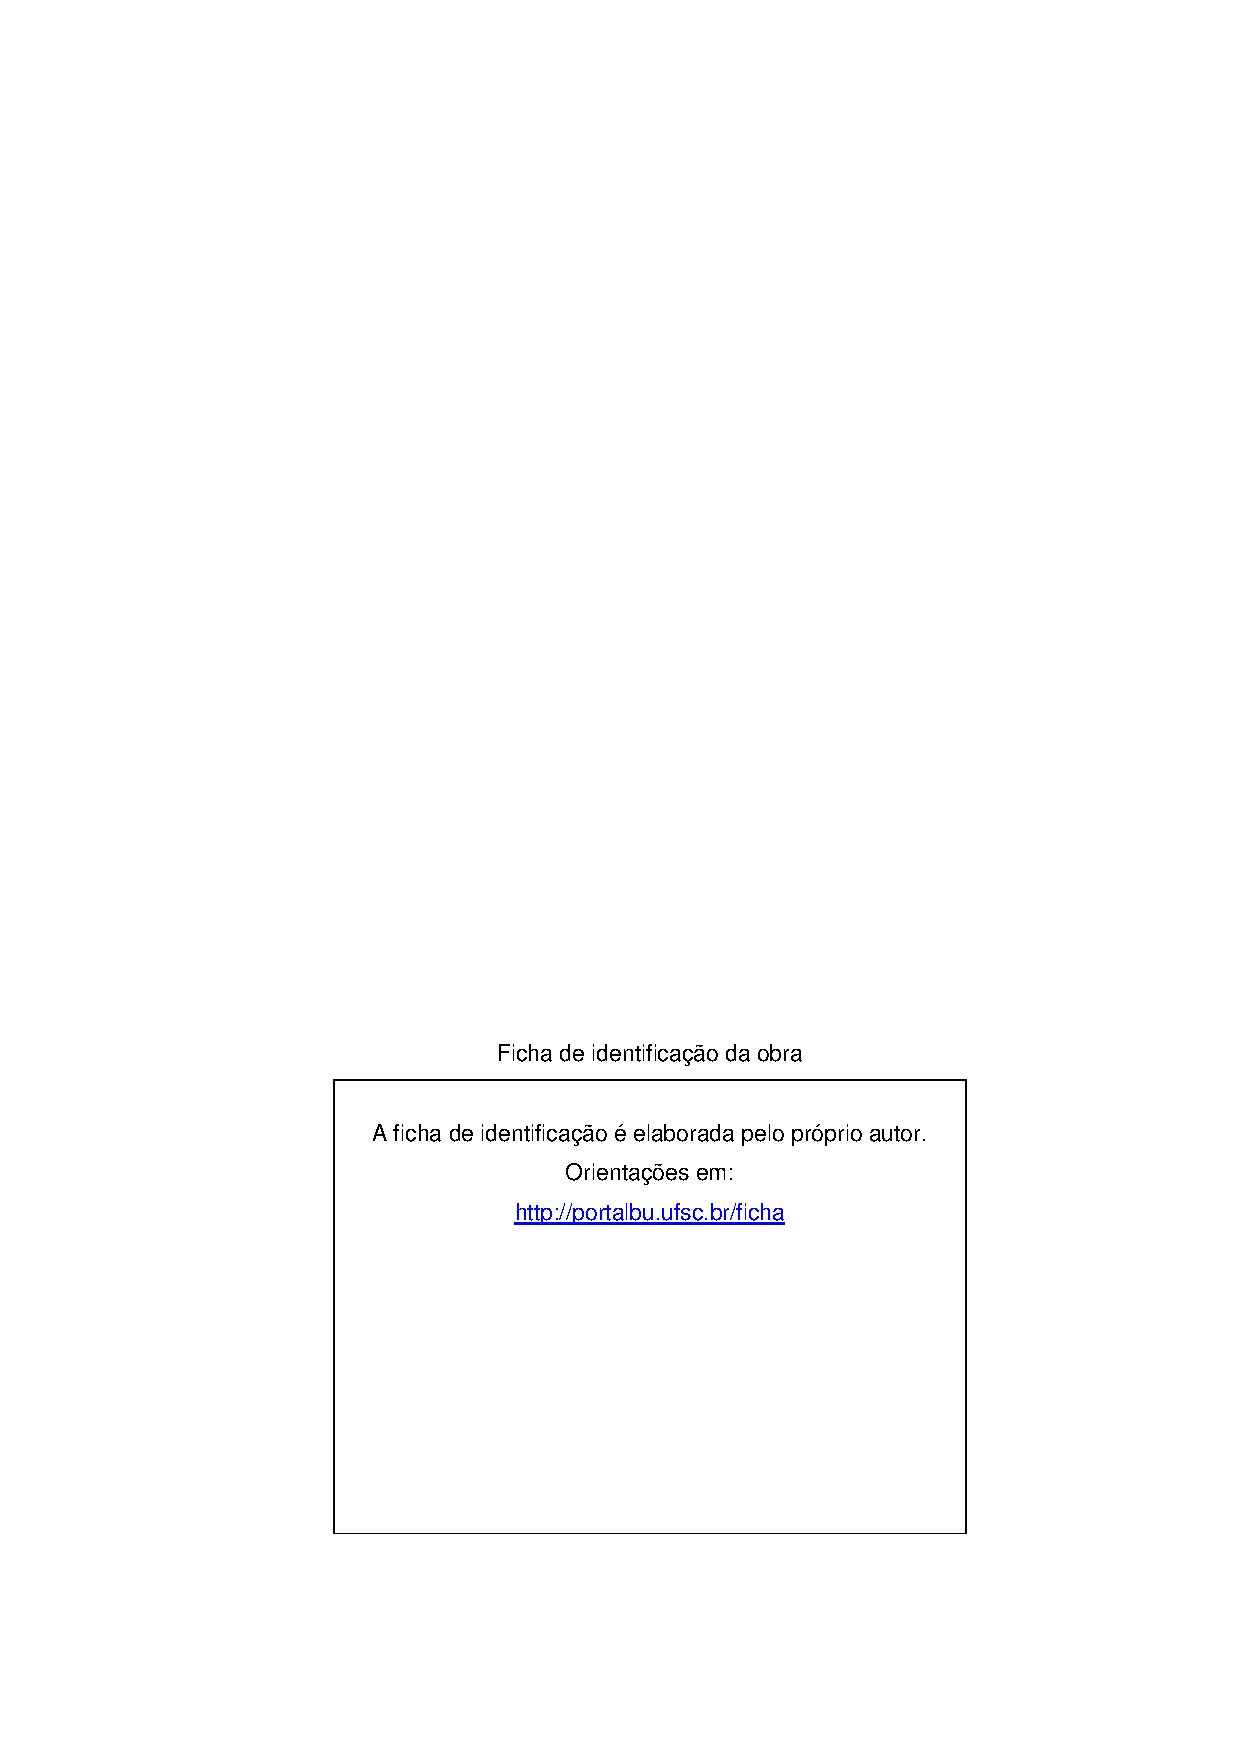
\includepdf{beforetext/Ficha_Catalografica.pdf}
\end{fichacatalografica}
% ---

% ---
% Inserir folha de aprovação
% ---
\begin{folhadeaprovacao}
	\OnehalfSpacing
	\centering
	\imprimirautor\\%
	\vspace*{10pt}		
	\textbf{\imprimirtitulo}%
	\ifnotempty{\imprimirsubtitulo}{:~\imprimirsubtitulo}\\%
	%		\vspace*{31.5pt}%3\baselineskip
	\vspace*{\baselineskip}
	%\begin{minipage}{\textwidth}
	% O presente trabalho em nível de \imprimirnivel~foi avaliado e aprovado por banca examinadora composta pelos seguintes membros
	The present work at \imprimirnivel~level was evaluated and approved by an examining board composed of the following members:\\
	%\end{minipage}%
	\vspace*{\baselineskip}
	Prof.(a) xxxx, Dr(a).\\
	Instituição xxxx\\
	\vspace*{\baselineskip}
	Prof.(a) xxxx, Dr(a).\\
	Instituição xxxx\\
	\vspace*{\baselineskip}
	Prof.(a) xxxx, Dr(a).\\
	Instituição xxxx\\
	\vspace*{2\baselineskip}
	\begin{minipage}{\textwidth}
		Certificamos que esta é a \textbf{versão original e final} do trabalho de conclusão que foi julgado adequado para obtenção do título de \imprimirformacao.\\
	\end{minipage}
	%    \vspace{-0.7cm}
	\vspace*{\fill}
	\assinatura{\OnehalfSpacing Coordenação do Programa de Pós-Graduação}
	\vspace*{\fill}
	\assinatura{\OnehalfSpacing\imprimirorientador \\ \imprimirorientadorRotulo}
	%	\ifnotempty{\imprimircoorientador}{
	%	\assinatura{\imprimircoorientador \\ \imprimircoorientadorRotulo \\
	%		\imprimirinstituicao~--~\imprimirinstituicaosigla}
	%	}
	% \newpage
	\vspace*{\fill}
	\imprimirlocal, \imprimirano.
\end{folhadeaprovacao}
% ---

% ---
% Dedicatória
% ---
\begin{dedicatoria}
	\vspace*{\fill}
	\noindent
	\begin{adjustwidth*}{}{5.5cm} 
		\raggedleft       
		Este trabalho é dedicado aos meus colegas de classe e aos meus queridos pais.
	\end{adjustwidth*}
\end{dedicatoria}
% ---

% ---
% Agradecimentos
% ---
\begin{agradecimentos}
	Inserir os agradecimentos aos colaboradores à execução do trabalho. 
	
	Xxxxxxxxxxxxxxxxxxxxxxxxxxxxxxxxxxxxxxxxxxxxxxxxxxxxxxxxxxxxxxxxxxxxxx. 
\end{agradecimentos}
% ---

% ---
% Epígrafe
% ---
\begin{epigrafe}
	\vspace*{\fill}
	\begin{flushright}
		\textit{``Texto da Epígrafe.\\
			Citação relativa ao tema do trabalho.\\
			É opcional. A epígrafe pode também aparecer\\
			na abertura de cada seção ou capítulo.\\
			Deve ser elaborada de acordo com a NBR 10520.''\\
			(SOBRENOME do autor da epígrafe, ano)}
	\end{flushright}
\end{epigrafe}
% ---

% ---
% RESUMOS
% ---

% resumo em português
\setlength{\absparsep}{18pt} % ajusta o espaçamento dos parágrafos do resumo
\begin{resumo}
	\SingleSpacing
	No resumo são ressaltados o objetivo da pesquisa, o método utilizado, as discussões e os resultados com destaque apenas para os pontos principais. O resumo deve ser significativo, composto de uma sequência de frases concisas, afirmativas, e não de uma enumeração de tópicos. Não deve conter citações. Deve usar o verbo na voz ativa e na terceira pessoa do singular. O texto do resumo deve ser digitado, em um único bloco, sem espaço de parágrafo. O espaçamento entre linhas é simples e o tamanho da fonte é 12. Abaixo do resumo, informar as palavras-chave (palavras ou expressões significativas retiradas do texto) ou, termos retirados de thesaurus da área. Deve conter de 150 a 500 palavras. O resumo é elaborado de acordo com a NBR 6028.
	
	\textbf{Palavras-chave}: Palavra-chave 1.  Palavra-chave 2. Palavra-chave 3.
\end{resumo}

% resumo em inglês
\begin{resumo}[Resumo]
	\SingleSpacing
	\begin{otherlanguage*}{english}
		Resumo traduzido para outros idiomas, neste caso, inglês. Segue o formato do resumo feito na língua vernácula. As palavras-chave traduzidas, versão em língua estrangeira, são colocadas abaixo do texto precedidas pela expressão “Keywords”, separadas por ponto.
		
		\textbf{Keywords}: Keyword 1. Keyword 2. Keyword 3.
	\end{otherlanguage*}
\end{resumo}

%% resumo em francês 
%\begin{resumo}[Résumé]
% \begin{otherlanguage*}{french}
%    Il s'agit d'un résumé en français.
% 
%   \textbf{Mots-clés}: latex. abntex. publication de textes.
% \end{otherlanguage*}
%\end{resumo}
%
%% resumo em espanhol
%\begin{resumo}[Resumen]
% \begin{otherlanguage*}{spanish}
%   Este es el resumen en español.
%  
%   \textbf{Palabras clave}: latex. abntex. publicación de textos.
% \end{otherlanguage*}
%\end{resumo}
%% ---

{%hidelinks
	\hypersetup{hidelinks}
	% ---
	% inserir lista de ilustrações
	% ---
	\pdfbookmark[0]{\listfigurename}{lof}
	\listoffigures*
	\cleardoublepage
	% ---
	
	% ---
	% inserir lista de quadros
	% ---
	\pdfbookmark[0]{\listofquadrosname}{loq}
	\listofquadros*
	\cleardoublepage
	% ---
	
	% ---
	% inserir lista de tabelas
	% ---
	\pdfbookmark[0]{\listtablename}{lot}
	\listoftables*
	\cleardoublepage
	% ---
	
	% ---
	% inserir lista de abreviaturas e siglas (devem ser declarados no preambulo)
	% ---
	\imprimirlistadesiglas
	% ---
	
	% ---
	% inserir lista de símbolos (devem ser declarados no preambulo)
	% ---
	\imprimirlistadesimbolos
	% ---
	
	% ---
	% inserir o sumario
	% ---
	\pdfbookmark[0]{\contentsname}{toc}
	\tableofcontents*
	\cleardoublepage
	
}%hidelinks
% ---
% ---

% ----------------------------------------------------------
% ELEMENTOS TEXTUAIS
% ----------------------------------------------------------
\textual


% ----------------------------------------------------------
\chapter{Introduction}
% ----------------------------------------------------------




% \section{Motivation and context}

% Context
According to the last report \textit{Justiça em Números}, published annually by the National Council of Justice (CNJ), by the end of 2019, there was around 77,1 million ongoing processes waiting for a solution in the Brazilian Judiciary. In total, in 2019, 30,2 million lawsuits were filled in all Judiciary, an increase of 6,8\% in relation to 2018. From those processes, about 5,2 million were filled in the Special Civel Courts (JECs)  \cite{CNJ2020}. 

% Write about JECs
JECS are Judiciary bodies regulated by Law no. 9,099/1995, which seek to facilitate citizens' access to Justice through simpler and cost-free procedures. As a result, JECs tend to approach the legal problems of ordinary people who find themselves involved in daily conflicts of small economic expression, whether in the purchases they make, in the services they hire or in the accidents they suffer \cite{Watanabe1985}.

% The increasing interest in applying legal judgements (cite RSL?)
Considering the challenges faced in the judiciary system in Brazil and around the world (CITE), there is an increasing interest (CITE) of the literature on applying Artificial Intelligence (AI) based techniques to solve issues from the lower courts (CITE), such as JECs, to the superior courts (CITE).

% What is AI?
AI, according to \textcite{Russell2020}, relates to the study of intelligent agents that receives percepts or inputs from the environment and make actions. The agent uses a function to map the percepts to the appropriate actions and such function can be explicitly defined and/or learned using Machine Learning (ML) techniques (CITE).

% ML tasks in the legal environment

\todo{Improve} In the legal context, the agent receives as percept (inputs) a the case's  textual data and acts (output) setting a decision. Considering the complexity of legal judgments, such decision may be learned using ML and Text Mining (TM) techniques, \todo{Define TM}.

% What is Classification, clustering and regression in this work?
Regarding the tasks to apply in legal decisions include clustering, which is ..., classification..., regression, ... (?)

% The many applications of TM and NLP
TM techniques have been used to solve several tasks regarding textual data, such as classification (CITE DEF), regression (CITE DEF) and clustering (CITE DEF) in several contexts, such as the legal (), medical (), engineering and social media

% NLP

\todo{Continue...}


% ----------------------------------------------------------
\section{Problem Definition} % Problem and Hypothesis
% ----------------------------------------------------------

% The importance of the JECS and the problem of 
The judicial lawsuits processed at the JECs are decided manually by the judge, and there is no automation in that sense. This leads to slowness and, as a consequence, the large number of processes pending solution (CITE). In addition, these processes are composed of unstructured textual data that, in addition to being represented in natural language, have their own legal vocabulary (CITE). 

% falar da RSL que foi feita e que vamos detalhar depois)

% 

\section{Research Question}

``Is it possible to predict the result of a legal case based on its content and predict the amount of compensation for immaterial damage using machine learning and text mining techniques?''

The question can be broke down into three:

\begin{itemize}[noitemsep]
    \item How to translate the complexity of the legal language to a numerical representation?
    \item Which machine learning techniques for classification can bring an legally acceptable accuracy to the predicted lawsuit result?
    \item Which machine learning techniques for regression can bring an legally acceptable error to the predicted amount of compensation for immaterial damage?
\end{itemize}

% ----------------------------------------------------------
\section{Objectives}
% ----------------------------------------------------------

In this section we introduce to the reader the main objective and the specific objectives necessary to achieve it.

% ----------------------------------------------------------
\subsection{Main Objective}
% ----------------------------------------------------------

To evaluate if we can predict with a legally acceptable amount of accuracy the result of a legal case and predict the amount of compensation using machine learning and text mining techniques.

% ----------------------------------------------------------
\subsection{Specific Objectives}
% ----------------------------------------------------------

To do that we need to:

\begin{itemize}[noitemsep]
    \item Demonstrate that representing the legal cases numerically using word embeddings and BOW can achieve legally acceptable results in the classification and regression tasks.
    \item Demonstrate that it is possible to predict the lawsuit result using classical and deep machine learning techniques for classification with legally acceptable accuracy.
    \item Demonstrate that it is possible to predict the amount of compensation  using classical and deep machine learning  techniques for regression with legally acceptable error.
\end{itemize}

% ----------------------------------------------------------
\section{Justification and Subject Relevance}
% ----------------------------------------------------------
\begin{itemize}[noitemsep]
    \item RSL Results
    \item AI Regulations and initiatives
    \item Growth in interest 
\end{itemize}

% ----------------------------------------------------------
\section{Methodological Procedures}
% ----------------------------------------------------------

\begin{itemize}[noitemsep]
    \item Systematic Review
    \item Legal Dataset 
    \item Experiments using Python
    \item Evaluation
    \item Check Legal Acceptable Accuracy and Errors
    \item Resources
\end{itemize}

% Structure
% Include here the research delimitation
% The steps we have followed to answer the question


% ----------------------------------------------------------

\section{Contributions}
% ----------------------------------------------------------

During the research, experiments were conducted to answer the research questions. Some of these experiments resulted in publications in journals and conferences. Considering the published works and the experiments applied, the contributions of these work are as follows:

\begin{itemize}[noitemsep]
    \item Pre-trained word embeddings models for Brazilian legal texts, since there was no available representation available before.
    \item Impact of adjustments in the pipeline for regression and classification.
    \item As real life application, we would help the Judiciary by helping to end the lawsuits in JEC at the conciliation hearing step.
\end{itemize}

% Contribuições mais acadêmicas
% Contribuições mais práticas
% - Help to speed up the process by ending them at the conciliation hearing.

% ----------------------------------------------------------
\section{Document Organization}
% ----------------------------------------------------------

The work is structured in X chapters, beginning with this introduction.

In \citechapter{cap:ml_text}, we introduce...

In \citechapter{cap:related_works}, ...







% ============================================================================================ %







% As orientações aqui apresentadas são baseadas em um conjunto de normas elaboradas pela \gls{ABNT}. Além das normas técnicas, a Biblioteca também elaborou uma série de tutoriais, guias, \textit{templates} os quais estão disponíveis em seu site, no endereço \url{http://portal.bu.ufsc.br/normalizacao/}.

% Paralelamente ao uso deste \textit{template} recomenda-se que seja utilizado o \textbf{Tutorial de Trabalhos Acadêmicos} (disponível neste link \url{https://repositorio.ufsc.br/handle/123456789/180829}) e/ou que o discente \textbf{participe das capacitações oferecidas da Biblioteca Universitária da UFSC}.

% Este \textit{template} está configurado apenas para a impressão utilizando o anverso das folhas, caso você queira imprimir usando a frente e o verso, acrescente a opção \textit{openright} e mude de \textit{oneside} para \textit{twoside} nas configurações da classe \textit{abntex2} no início do arquivo principal \textit{main.tex} \cite{abntex2classe}.

% Conforme a \href{https://repositorio.ufsc.br/bitstream/handle/123456789/197121/RN46.2019.pdf?sequence=1&isAllowed=y}{Resolução NORMATIVA nº 46/2019/CPG} as dissertações e teses não serão mais entregues em formato impresso na Biblioteca Universitária. Consulte o Repositório Institucional da UFSC ou sua Secretaria de Pós Graduação sobre os procedimentos para a entrega. 

% \nocite{NBR6023:2002}
% \nocite{NBR6027:2012}
% \nocite{NBR6028:2003}
% \nocite{NBR10520:2002}

% % ----------------------------------------------------------
% \section{Objetivos}
% % ----------------------------------------------------------

% Nas seções abaixo estão descritos o objetivo geral e os objetivos 
% específicos.

% % ----------------------------------------------------------
% \subsection{Objetivo Geral}
% % ----------------------------------------------------------

% Descrição...

% % ----------------------------------------------------------
% \subsection{Objetivos Específicos}
% % ----------------------------------------------------------

% Descrição...
% ----------------------------------------------------------
\chapter{Machine Learning for Text}\label{cap:ml_text}

\section{Machine Learning (definição)}

\section{Text Mining and Natural Language Processing}

\begin{itemize}
    \setlength\itemsep{-0.5em}
    \item Definição de Text Mining e NLP
    \item Como se enquadram no trabalho
    \item Aplicações
\end{itemize}

\section{Text Pré-Processing}

Filtering, Lowercasing, Stopwords, etc.

\section{Text Representation}

\subsection{Bag of Words}

\subsection{Word Embeddings}

\subsection{Recent techniques (n usadas; BERT, GPT-3, ...)}

\section{Classification}

\subsection{Definition}

\subsection{Techniques}

\subsection{Evaluation Methods}

\subsection{Applications in Textual Data}

\section{Regression}

\subsection{Definition}

\subsection{Techniques}

\subsection{Evaluation Methods}


\subsection{Applications in Textual Data}


\section{Conclusions for the Chapter}
% % ----------------------------------------------------------

% ----------------------------------------------------------
\chapter{Related Works}\label{cap:related_works}
% ----------------------------------------------------------


\section{Related works in Text Representation}


\section{Related works in Text Classification}


\section{Related works in Text Regression}


\section{Conclusions for the Chapter}

% ----------------------------------------------------------
\chapter{Machine Learning in Brazilian Legal Cases}
% ----------------------------------------------------------

% ----------------------------------------------------------
\section{Numerical Representations of Legal Texts}
% ----------------------------------------------------------

% \subsection{Introduction}

% \subsection{Dataset (Context, Acquisition, Quali, Quant info)}

% \subsection{Embeddings Training}

% \subsection{Evaluation on Text Classification}


% ----------------------------------------------------------
\section{Classification on Legal Texts}
% ----------------------------------------------------------

% \subsection{Introduction}

% \subsection{Dataset (Context, Acquisition, Quali, Quant info)}

% \subsection{Pipeline}

% \subsection{Evaluation}




% ----------------------------------------------------------
\section{Regression on Legal Texts}
% ----------------------------------------------------------

%\subsection{Introduction}

%\subsection{Dataset (Context, Acquisition, Quali, Quant info)}

%\subsection{Pipeline (Ajustes)}

%\subsection{Evaluation}

% ----------------------------------------------------------
%\section{Conclusions for the Chapter}
% ----------------------------------------------------------
% ----------------------------------------------------------
\chapter{Final Remarks}
% ----------------------------------------------------------

\section{Technical Production (Artigos)}

\begin{flushleft}

SABO, Isabela Cristina; DAL PONT, Thiago Raulino; ROVER, Aires José; HÜBNER, Jomi Fred. Classificação de sentenças de Juizado Especial Cível utilizando aprendizado de máquina. \textbf{Revista Democracia Digital e Governo Eletrônico}, v. 1, n. 18, p. 94–106, 2019.

\vspace{1em}

DAL PONT, Thiago Raulino; SABO, Isabela Cristina; HÜBNER, Jomi Fred; ROVER, Aires José. Impact of Text Specificity and Size on Word Embeddings Performance: An Empirical Evaluation in Brazilian Legal Domain. In: CERRI, Ricardo; PRATI, Ronaldo C. (Eds.). Cham: Springer International Publishing, 2020. v. 12319. (Lecture Notes in Computer Science). P. 521–535. DOI:10.1007/978-3-030-61377-8\_36. 

\vspace{1em}

SABO, Isabela Cristina; DAL PONT, Thiago Raulino; WILTON, Pablo Ernesto Vigneaux; ROVER, Aires José; HÜBNER, Jomi Fred. Clustering of Brazilian legal judgments about failures in air transport service: an evaluation of different approaches. \textbf{Artificial Intelligence and Law}, Springer Netherlands, n. 0123456789, p. 1–37, Apr. 2021. ISSN 0924-8463. DOI:10.1007/s10506-021-09287-3.

\vspace{1em}


(Submitted) 
\end{flushleft}


\section{Limitations}

\section{Future Work}


\section{Extra Information (Git)}

\section{Acknowledgement (para CAPES e Petrobras)}


% ----------------------------------------------------------
% ELEMENTOS PÓS-TEXTUAIS
% ----------------------------------------------------------
\postextual
% ----------------------------------------------------------

% ----------------------------------------------------------
% Referências bibliográficas
% ----------------------------------------------------------
\begingroup
    \printbibliography[title=REFERENCES]
\endgroup

% ----------------------------------------------------------
% Glossário
% ----------------------------------------------------------
%
% Consulte o manual da classe abntex2 para orientações sobre o glossário.
%
%\glossary

% ----------------------------------------------------------
% Apêndices
% ----------------------------------------------------------

% ---
% Inicia os apêndices
% ---
\begin{apendicesenv}
%	\partapendices* 
	% ----------------------------------------------------------
\chapter{Systematic Review of the Literature: AI, ML and Law} \label{ap:rsl_ml_law}
% ----------------------------------------------------------

The Systematic Review of the Literature, detailed in this section, focused on finding works related to the applications of TM and ML in the legal domain.


\section{Definition of Search Questions}

The main question in this SRL is: ``Which are the Text Mining Techniques applied in the legal domain?''

As secondary questions, there is:

\begin{itemize}[noitemsep]
    \item Which is the legal application?
    \item What are the pre-processing techniques used?
    \item What are the representation techniques used?
    \item What are the feature extraction techniques used?
    \item What are the classification techniques used?
    \item What are the clustering techniques used?
    \item What are the regression techniques used?
    \item What are the evaluation techniques used?
\end{itemize}

\section{Search Strategies}

In order to have an overview of the publications regarding TM and legal domain, we searched in February 29, 2020, for works published on conferences or journals from 2010 to 2020.  The search used the following search string:

\begin{verbatim}
    ("text mining" OR "natural language processing" OR "nlp" OR
    "language processing") AND ("deep learning" OR "machine learning")
    AND ("classification" OR "cluster*" OR "regression" OR 
    "categorization" OR "embedding*" OR "representation" OR "predict*")
    AND ("text" OR "document") AND ("law" OR "legal" OR "judicial" OR
    "justice" OR "court" OR "legislation" OR "juridical" OR "lawful")
\end{verbatim}

In this search, we also added synonymous for Machine Learning, Text Mining, and ML Tasks, and the legal domain.

The search embraced the papers' titles, abstracts and keywords.

\section{Knowledge Bases}

In this SRL, we included bases predominantly related to computing as well as interdisciplinary basis.  The list of knowledge bases follows:

\begin{itemize}[noitemsep]
    \item Scopus
    \item IEEE Xplore
    \item Web of Science
    \item ACM Digital Library
\end{itemize}

\section{Inclusion and Exclusion Criteria}

Following the questions of this research, we defined a set of inclusion and exclusion criteria. The process of selection embraced the reading of title, abstract and keywords and the accordance with the criteria:

The following is the list of inclusion criteria:

\begin{itemize}[noitemsep]
    \item Published in journal or conference
    \item Involves legal processes, or texts with juridical language;
    \item Involves Machine Learning or Text Mining;
    \item The techniques used are named;
    \item Empirical Works.
    \item Published from 2010 and February 2020.
\end{itemize}

And the following is the list of exclusion criteria:

\begin{itemize}[noitemsep]
    \item Not written in Portuguese or English;
    \item Published over 10 years ago;
    \item Does not involve Machine Learning or Text Mining;
    \item Does not involve the legal domain;
    \item Theoretical works.
\end{itemize}


\section{Data Extraction Plan}

Information to extract from the papers:

\begin{itemize}[noitemsep]
    \item Title
    \item Keywords
    \item Abstract
    \item Authors
    \item Year of publication
    \item Journal or Conference
    \item Authors affiliation
    \item Pre-processing techniques
    \item Representation / Feature Extraction Techniques
    \item Classification  / Clustering / Regression Techniques
    \item Other techniques
    \item Model Evaluation Techniques
\end{itemize}


\section{Search Execution and Preliminary Analysis}

After applying the search strings to the knowledge bases on February 29, 2020 without filters on year of publication, we obtained the number of publications shown in Figure \ref{fig:ap_rsl_tm_law}.

\begin{figure}[H]
    \centering
    \caption{Publications on ML and TM applied to the legal domain from 2000 to 2019}
    \label{fig:ap_rsl_tm_law}
    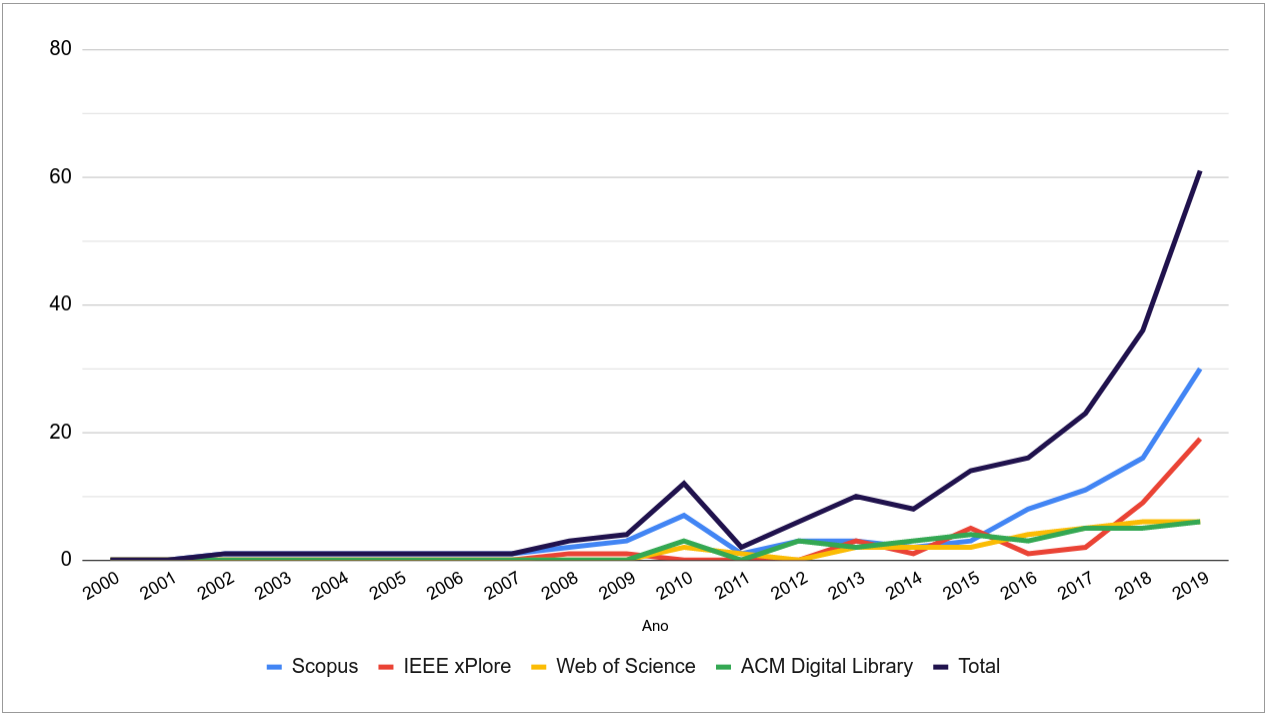
\includegraphics[width=\textwidth]{images/appendix/artigos_tm_law.png}
\end{figure}

After applying the search strings to the knowledge bases with time filtering on February 29, 2020, the search returned 195. After duplicates removal, the number of works reduced to 147. Finally, from the reading of title, abstract and keywords and the application of the selection criteria, the number of works selected for full reading reduced to 46.

The selected works were used as references in the Introduction chapter, in the Related Works and in the Background.

\section{Results and Analysis}
In this section we show a sequence of quantitative data in terms of the tens most frequent authors, journals, text mining techniques and others.

In the following tables, there is ten most frequent authors and conferences found in the SRL and the most frequent techniques for pre-processing, representation, classification, clustering and evaluation.

% Legal Applications?

% Authors

\begin{table}[H]
    \footnotesize
    \centering
    \caption{Ten most frequent authors}
    \label{tab:rsl_freq_authors}
    \begin{tabular}{@{}cc@{}}
    
    \toprule
    \textbf{Authors}     & \textbf{Papers} \\ \midrule
    Matthes, Florian     & 5               \\
    Glaser, Ingo         & 4               \\
    Chalkidis, Ilias     & 3               \\
    Scepankova, Elena    & 3               \\
    Quaresma, Paulo      & 2               \\
    Gonçalves, Teresa    & 2               \\
    Galgani, Filippo     & 2               \\
    Compton, Paul        & 2               \\
    Hoffmann, Achim      & 2               \\
    Androutsopoulos, Ion & 2               \\ \bottomrule
    
    \end{tabular}
\end{table}

% Journals / Conferences

\begin{table}[H]
\footnotesize
    \centering
    \caption{Ten most frequent journals and conferences}
    \label{tab:rsl_freq_conferences}
\begin{tabular}{@{}p{14cm}c@{}}
\toprule
\multicolumn{1}{c}{\textbf{Journal / Conference}}                                                         & \textbf{Papers} \\ \midrule
Lecture Notes in Computer Science                                                                         & 8               \\
CEUR Workshop Proceedings                                                                                 & 4               \\
Frontiers in Artificial Intelligence and Applications                                                     & 3               \\
Artificial Intelligence and Law                                                                           & 2               \\
2010 6th International Conference on Wireless Communications, Networking and Mobile Computing, WiCOM 2010 & 1               \\
Proceedings of the ACM Conference on Computer and Communications Security                                 & 1               \\
Foundations and Trends in Information Retrieval                                                           & 1               \\
Conference on Legal Knowledge and Information Systems                                                     & 1               \\
Expert Systems with Applications                                                                          & 1               \\
International Conference on Cloud Computing and Services Science                                          & 1               \\ \bottomrule
\end{tabular}
\end{table}

% Pré-processing Techniques


\begin{table}[H]
\centering
\footnotesize
\caption{Ten most frequent pre-processing techniques}
\label{tab:rsl_freq_pre_processing}

    \begin{tabular}{@{}ll@{}}
    
    \toprule
    \multicolumn{1}{c}{\textbf{Preprocessing}} & \multicolumn{1}{c}{\textbf{Papers}} \\ \midrule
    Stop words removal                         & 15                                  \\
    Lemmatization                              & 8                                   \\
    Stemming                                   & 7                                   \\
    Tokenization                               & 4                                   \\
    Lowercase                                  & 4                                   \\
    POS Tagging                                & 3                                   \\
    Normalization                              & 3                                   \\
    Remove punctuation                         & 3                                   \\
    Remove noise                               & 1                                   \\
    Regularization                             & 1                                   \\ \bottomrule
    
    \end{tabular}
\end{table}


% Representation Techniques
\begin{table}[H]
\centering
\footnotesize
\caption{Ten most frequent representation techniques}
\label{tab:rsl_freq_representation}
\begin{tabular}{@{}lc@{}}
\toprule
\textbf{Representation}  & \textbf{Papers} \\ \midrule
TF-IDF                   & 19              \\
Word2Vec                 & 14              \\
Bag of Words             & 10              \\
N-Gram                   & 7               \\
Part-of-Speech Tag       & 6               \\
Named Entity Recognition & 5               \\
Doc2Vec                  & 4               \\
Word Embeddings          & 3               \\
FastText                 & 3               \\ 
BERT                     & 2               \\ \bottomrule
\end{tabular}
\end{table}

% Classification techniques
\begin{table}[H]
\centering
\footnotesize
\caption{Ten most frequent classification techniques}
\label{tab:rsl_freq_classification}
\begin{tabular}{@{}cc@{}}
\toprule
\textbf{Classification Tech} & \textbf{Papers} \\ \midrule
Support Vector Machine       & 24              \\
Convolution Neural Network   & 19              \\
Naïve Bayes                  & 18              \\
Decision Tree                & 17              \\
k Nearest Neighbors          & 14              \\
Recurrent neural network     & 14              \\
Random Forest                & 13              \\
Long Short Term Memor y      & 13              \\
Logistic Regression          & 11              \\
Conditional Random Field     & 7               \\ \bottomrule
\end{tabular}
\end{table}


% Clustering Techniques
\begin{table}[H]
\centering
\caption{Most frequent clustering techniques}
\label{tab:rsl_freq_clustering}
\footnotesize
\begin{tabular}{cc}
\hline
\textbf{Clustering Tech} & \textbf{Papers} \\ \hline
Hierarchical Clustering  & 2               \\
Fuzzy C-Means            & 1               \\
Hierarchical LDA         & 1               \\
k-Means                  & 1              \\
\bottomrule
\end{tabular}
\end{table}

\begin{table}[H]
\centering
\caption{Ten most frequent evaluation metrics}
\label{tab:rsl_freq_evaluation}
\footnotesize
\begin{tabular}{cc}
\hline
\textbf{Evaluation Metric} & \textbf{Papers} \\ \hline
F1-score                   & 23              \\
Accuracy                   & 21              \\
Precision                  & 20              \\
Recall                     & 19              \\
Cross-validation           & 6               \\
Rouge                      & 2               \\
Area under curve ROC       & 2               \\
ROC                        & 1               \\
BLEU                       & 1               \\ \bottomrule
\end{tabular}
\end{table}



% Regression Techniques
This SRL did not find works that applied regression techniques in the legal domain.





	% ----------------------------------------------------------
\chapter{Systematic Review of the Literature: Text Representation}\label{ap:rsl_representation_law}
% ----------------------------------------------------------


% - Focus on word embeddings and language models
% - 

In this SRL, we tried to find work related to the application of text representation techniques on legal texts written in the Portuguese language. However, such task did not succeed due to the absence of work in that sense. Thus, two smaller SRLs were conducted to find papers with broader searches. The first focused on the representation of legal texts in any language and the second in the representation of general texts in Portuguese. 

\section{Definition of Search Questions}

The question of the first search: ``What are the text representation techniques applied to texts from the legal domain?''

The question of the second search: ``What are the text representation techniques applied to texts written in Portuguese?''

\section{Search Strategies}

Search for representation of legal texts in any languages:

\begin{verbatim}
("legal" OR "law" OR "court" OR "justice") AND ("embedding*" OR 
"language model*" OR "machine learning" OR "deep learning" OR 
"natural language processing" OR "text mining") AND ("doc2vec" 
OR "paragraph2vec" OR "word2vec" OR "glove" OR "wang2vec" OR 
"fasttext" OR "bert" OR "elmo" OR "law2vec")
\end{verbatim}


Search for representation of general texts in Portuguese:

\begin{verbatim}
("portuguese" OR "brazil*") AND ("embedding*" OR "deep learning" OR 
"machine learning" OR "natural language processing" OR "text mining") 
AND ("doc2vec" OR "paragraph2vec" OR "word2vec" OR "glove" OR 
"wang2vec" OR "fasttext" OR "bert" OR "elmo" OR "law2vec" ) 
\end{verbatim}



\section{Knowledge Bases}

In this SRL, we searched on the following bases:

\begin{itemize}[noitemsep]
    \item Scopus
    \item ACM Digital Library
    \item IEEE Xplore
    \item Web of Science
\end{itemize}


\section{Inclusion and Exclusion Criteria}


Following the questions of this research, we defined a set of inclusion and exclusion criteria. The process of selection embraced the reading of title, abstract and keywords and the accordance with the criteria:

The following is the list of inclusion criteria:

\begin{itemize}[noitemsep]
    \item Published in journal or conference
    \item Involves legal texts in any languages or general texts in Portuguese;
    \item Involves Machine Learning or Text Mining;
    \item The techniques used are named;
    \item The work evaluate or train representations
    \item Empirical Work;
    \item Published from 2010 and May 2020.
\end{itemize}

And the following is the list of exclusion criteria:

\begin{itemize}[noitemsep]
    \item Work not written in Portuguese or English;
    \item Published over 10 years ago;
    \item Does not involve legal texts in any language neither general texts in Portuguese;
    \item Does not involve Machine Learning or Text Mining;
    \item Theoretic work
\end{itemize}

\section{Data Extraction Plan}

In the SRL from this section, we focused on just retrieving the representation techniques used and the application.

\section{Search Execution and Preliminary Analysis}

After applying the first search string to the knowledge base on May 7, 2020 for researches published from 2010 to May 2020, the search returned 52 documents. After reading title, abstract and keywords and applying the selection criteria, the number of papers reduced to 12.

In terms of the second search string, after applying to the knowledge base on May 7, 2020 with the same time filtering, the search returned 136 documents. After reading title, abstract and keywords and applying the selection criteria, the number of papers reduced to 20.


\section{Results and Analysis}

In this section, we show the results and analysis in terms of representation techniques for the first part of this SRL related to legal texts from many languages and general texts in Portuguese.

In the first part of this research, we focused on the representation techniques applied in the legal domain. In Figure \ref{fig:rsl_legal_representation}, one can see the distribution by year of the research interest, on the area of representation of legal documents for ML tasks, considering our selection criteria. Although we set the interval to ten years, the selected work only embraced three distinct years.


\begin{figure}[htb]
    \centering
    \caption{Researches by year for text representation in legal documents}
    \label{fig:rsl_legal_representation}
    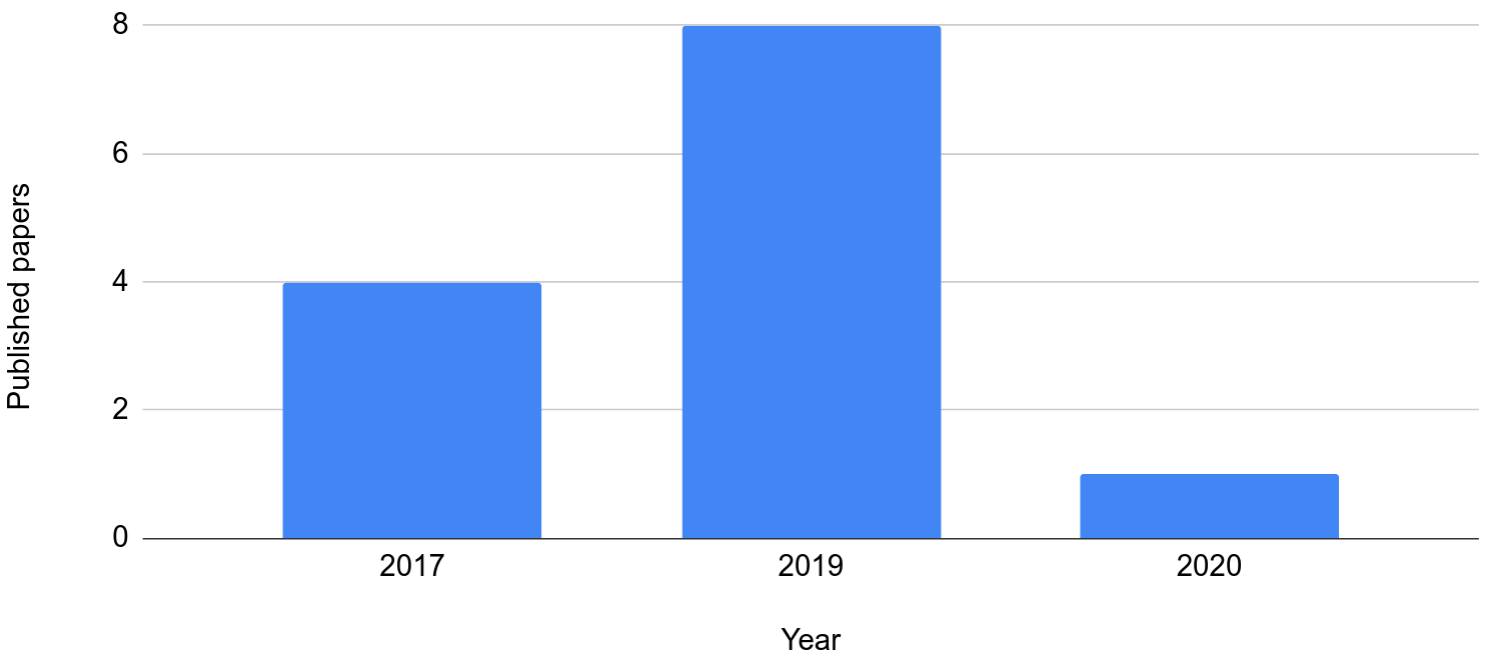
\includegraphics[width=\textwidth]{images/appendix/rsl_legal_representation.png}
\end{figure}

In Table \ref{tab:rsl_representation_legal}, there is the list of representation techniques used in the selected work. Note that, many papers reported using more than one representation techniques in their experiments.

% Most frequent Representations
\begin{table}[htb]
\centering
\caption{Representations applied to legal texts}
\label{tab:rsl_representation_legal}
\footnotesize
\begin{tabular}{cc}
\hline
\textbf{Representation} & \textbf{Papers} \\ \hline
Word2Vec                & 8               \\
Doc2Vec                 & 2               \\
WordVec CBOW           & 2               \\
Glove                   & 2               \\
FastText                & 2               \\
ELMo                    & 1               \\
Bag of Words            & 1               \\
Law2Vec                 & 1              \\\bottomrule
\end{tabular}
\end{table}

In the second part of this research, we focused on the representation techniques applied in general texts written in the Portuguese language. In Figure \ref{fig:rsl_representation_portuguese_year}, one can see the distribution by year of the research interest on the area, considering our selection criteria. Although, the SRL embraced the last ten years the selected work embraced the last five.


\begin{figure}[htb]
    \centering
    \caption{Researches by year for text representation in Portuguese documents}
    \label{fig:rsl_representation_portuguese_year}
    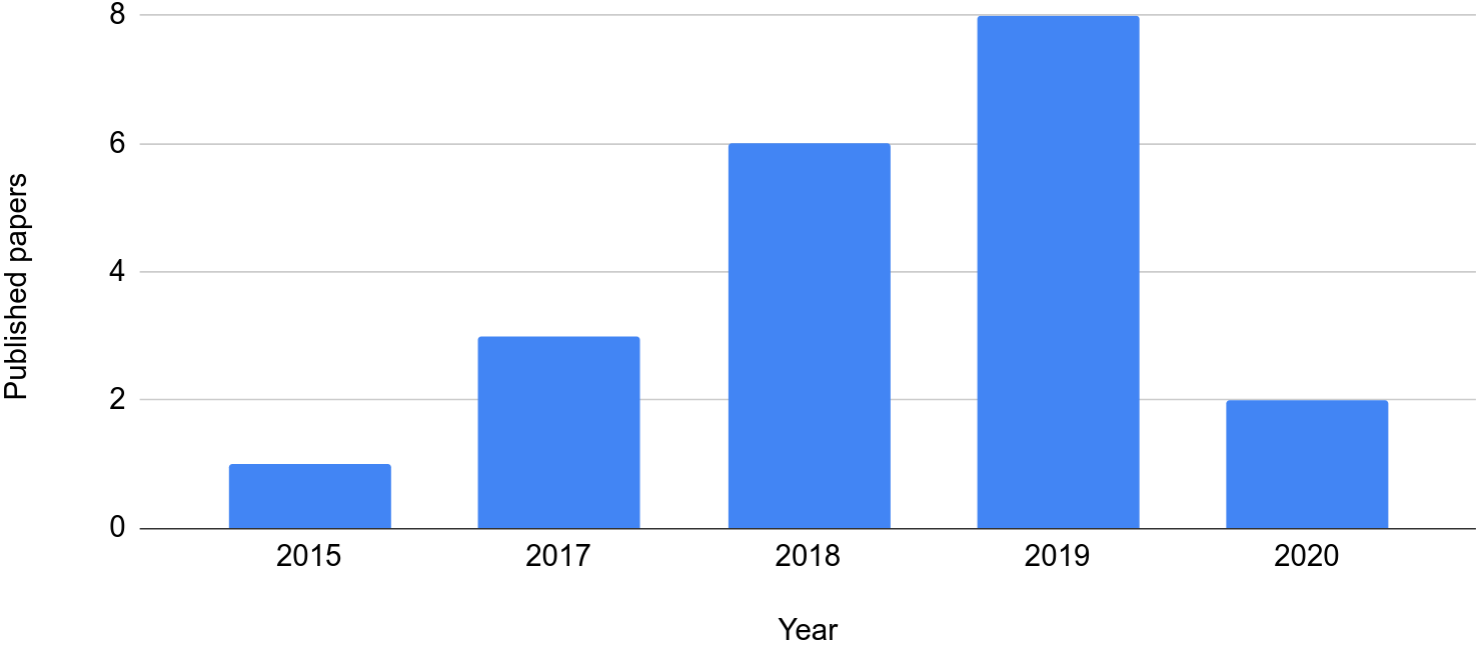
\includegraphics[width=\textwidth]{images/appendix/rsl_portuguese_representation.png}
\end{figure}

In Table \ref{tab:rsl_representation_portuguese}, there is the list of representation techniques used in the selected work. Note that, many papers reported using more than one representation techniques in their experiments.

\begin{table}[htb]
\centering
\caption{Representation used in Portuguese texts}
\label{tab:rsl_representation_portuguese}
\footnotesize
\begin{tabular}{cc}
\hline
\textbf{Representation} & \textbf{Papers} \\ \hline
Word2Vec                & 7               \\
Word2Vec Skipgram       & 7               \\
Glove                   & 6               \\
TF-IDF                  & 3               \\
Wang2Vec Skipgram       & 3               \\
Bag of Words            & 2               \\
ELMo                    & 2               \\
FastText                & 2               \\
FastText Skipgram       & 2               \\
LDA                     & 2              \\ \bottomrule
\end{tabular}
\end{table}

% Tasks

As mentioned, we do not find, until the date of the SRLs, any work related to evaluation or training of representations of  legal texts in the Portuguese language.


	% ----------------------------------------------------------
\chapter{Systematic Review of the Literature: Text Regression}\label{ap:rsl_regression_law}
% ----------------------------------------------------------

In this SRL, we focused on finding papers related to the application of regression techniques on legal texts written in the Portuguese language. However, such a task did not succeed due to the lack of work in that matter. Thus, we applied a broader search regarding the application of regression in texts without context or language limitations.

\section{Definition of Search Questions}

The question of this search is: ``What are the regression techniques applied to texts considering any applications and languages?''

\section{Search Strategies}

The search used the following search string:

% TODO: Continue from here.
\begin{verbatim}
  ( "regression on text*"  OR  "text* regression"  OR  "regression text*"  
  OR  "regression from text*"  OR  "regression for text*" )  
  AND NOT  "logistic regression"  
\end{verbatim}



\section{Search Resources}
In this SRL, we searched on the following bases:

\begin{itemize}[noitemsep]
    \item Scopus
    \item ACM Digital Library
    \item IEEE Xplore
    \item Web of Science
\end{itemize}

\section{Selection Criteria}

Following the questions of this research, we defined a set of inclusion and exclusion criteria. The process of selection embraced the reading of title, abstract and keywords, and the accordance with the criteria.

The following is the list of inclusion criteria:

\begin{itemize}[noitemsep]
    \item Published in journal or conference
    \item Involves regression applied to textual data;
    \item Involves Machine Learning or Text Mining;
    \item The techniques used are named;
    \item Empirical Work;
    \item Published from 2010 and December 2020.
\end{itemize}

And the following is the list of exclusion criteria:

\begin{itemize}[noitemsep]
    \item Work not written in Portuguese or English;
    \item Published over 10 years ago;
    \item Does not involve regression applied to textual data;
    \item Does not involve Machine Learning or Text Mining;
    \item Theoretic work.
\end{itemize}

\section{Data Extraction}
In the SRL from this section, we focused on retrieving the text representation, the regression techniques used and the evaluation metrics.

\section{Search Execution and Preliminary Analysis}

After applying the first search string to the knowledge base on December 1, 2020 for researches published from 2010 to December 2020, the search returned 124 documents. After reading title, abstract and keywords and applying the selection criteria, the number of papers reduced to 18.


\section{Results and Discussion}

% Técnicas mais comuns

In this section, we show the results and analysis in terms of regression techniques applied to text. In this part of this research, we focused on the regression techniques applied in any domains. In Figure \ref{fig:rsl_regression_year_publishing}, one can notice the distribution by year of the research interest on the area of the regression applied to texts.

% Publicações por ano

\begin{figure}[htb]
    \centering
    \caption{Papers published by year}
    \label{fig:rsl_regression_year_publishing}
    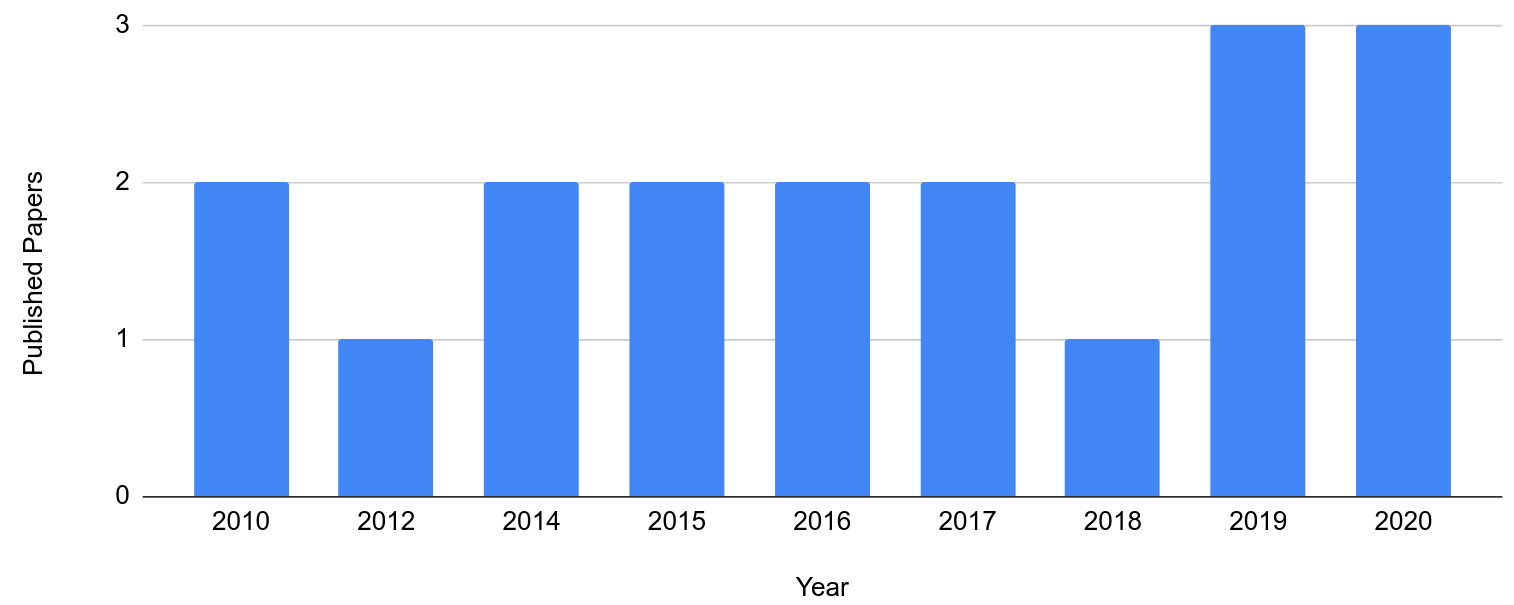
\includegraphics[width=\textwidth]{images/appendix/rsl_regression.png}
\end{figure}


In Table \ref{tab:rsl_regression_representation}, there are the representation techniques used in the selected work from the SRL. The most common technique is the Bag of Words followed by the N-Grams and TF-IDF, that is Vector Space Models representations. There is also neural based techniques such as word embeddings.


\begin{table}[htb]
\centering
\caption{Representation techniques in papers from regression SRL}
\label{tab:rsl_regression_representation}
\footnotesize
\begin{tabular}{@{}cc@{}}
\toprule
\textbf{Representation} & \textbf{Papers} \\ \midrule
Bag of Words & 8 \\
N-gram & 4 \\
TF-IDF & 4 \\
Metadata & 2 \\
Part-of-Speech Tag & 2 \\
Word Embeddings & 2 \\
Context ependence & 1 \\
Dependency relations & 1 \\
LDA & 1 \\
LSA & 1 \\ \bottomrule
\end{tabular}
\end{table}


In Table \ref{tab:rsl_regr_tech}, there are the most frequent regression techniques applied in the selected work. The most common is the Support Vector Machine, followed by Linear Regression, Convolution Neural Network, Elastic Net, Gaussian Copula, and Gradient Boosting.

\begin{table}[htb]
\centering
\caption{Regression techniques applied in the  papers from SRL}
\label{tab:rsl_regr_tech}
\footnotesize
\begin{tabular}{@{}lc@{}}
\toprule
\multicolumn{1}{c}{\textbf{Regression Tech}} & \textbf{Papers} \\ \midrule
Support Vector Machine & 7 \\
Linear Regression & 5 \\
Convolutional Neural Network & 2 \\
Elastic Net & 2 \\
Gaussian Copula & 2 \\
Gradient Boosting & 2 \\
Conditional Generative Adversarial Network & 1 \\
Gaussian Process & 1 \\
kNN & 1 \\
Lasso & 1 \\
Multinomial logistic text regression & 1 \\
Random Forest & 1 \\
Ridge & 1 \\
XGBoosting & 1 \\ \bottomrule
\end{tabular}
\end{table}

In Table \ref{tab:rsl_regr_evaluation}, there are the most common evaluation metrics for regression applied in the select work. One can note the Mean Absolute Error (MAE) is the most common, followed by Mean Square Error (MSE) and Root Mean Square Error (RMSE).

\begin{table}[htb]
\centering
\caption{Evaluation metrics for regression}
\label{tab:rsl_regr_evaluation}
\footnotesize
\begin{tabular}{@{}lc@{}}

\toprule
\multicolumn{1}{c}{\textbf{Evaluation Metric}} & \textbf{Papers} \\ \midrule
Mean Absolute Error & 9 \\
Mean Square Error & 3 \\
Root Mean Square Error & 3 \\
Pearson's correlation & 2 \\
Relative Absolute Error & 2 \\
Root Relative Squared Error & 2 \\
Adjusted R2 & 1 \\
F-variation & 1 \\
Kendall's Tau & 1 \\
R$^2$ & 1 \\
RAE & 1 \\
Spearman's Correlation & 1 \\
Standardization on Beta & 1 \\
Symmetric Mean Absolute Percentage Error & 1 \\
Value of $t$ & 1 \\ \bottomrule
\end{tabular}
\end{table}


\end{apendicesenv}
% ---


% ----------------------------------------------------------
% Anexos
% ----------------------------------------------------------

% ---
% Inicia os anexos
% ---
\begin{anexosenv}
%	\partanexos*
	% % ----------------------------------------------------------
% \chapter{Descrição 2}
% % ----------------------------------------------------------

% São documentos não elaborados pelo autor que servem como fundamentação (mapas, leis, estatutos). Deve ser precedido da palavra ANEXO, identificada por letras maiúsculas consecutivas, travessão e pelo respectivo título. Utilizam-se letras maiúsculas dobradas quando esgotadas as letras do alfabeto. 

\end{anexosenv}

%---------------------------------------------------------------------
% INDICE REMISSIVO
%---------------------------------------------------------------------
%\phantompart
%\printindex
%---------------------------------------------------------------------

\end{document}
